\chapter{Estado del Arte}
\label{cap:Estado-del-Arte}

En este capítulo se tratará el contexto tecnológico referente al trabajo en cuestión. Además, se pretende que sea también ilustrativo, dando una buena introducción a los conceptos y tecnologías a tratar en este documento. Esto es de gran relevancia para poder alimentar el marco teórico de este trabajo, y aclarar los conceptos desde donde se abordan las explicaciones en la investigación de este trabajo. 

\section{Dispositivos ARM}

\ac{ARM} \cite{arm1} \cite{arm2} es una arquitectura de microprocesadores enfocados en bajo consumo, basada en la filosofía \ac{RISC}. En sus inicios, \ac{ARM} iba dirigida a aquellos dispositivos alimentados por baterías, los cuales requieren un bajo consumo para alargar tanto como posible la vida de sus baterías, como \textit{smarpthones} o portátiles. Sin embargo, en la actualidad, el uso de procesadores \ac{ARM} se ha extendido a múltiples escenarios, abarcando una amplia gama de dispositivos, desde servidores hasta supercomputadores. \ac{ARM} ha demostrado ser una fuerza disruptiva en la industria de los procesadores, siendo una auténtica revolución en la computación. Un ejemplo de procesador \ac{ARM} se muestra en la figura \ref{procesadorArm}.

\begin{figure}[t]
    \centering
    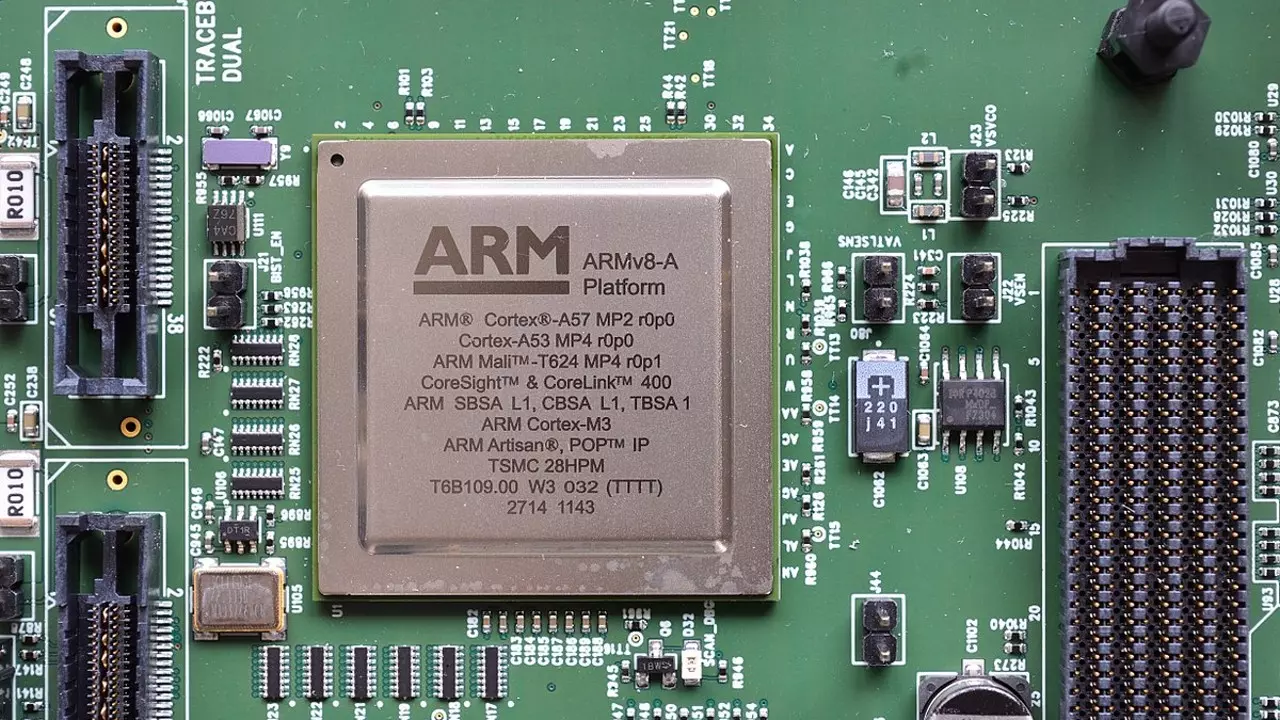
\includegraphics[width=0.5\linewidth, height=0.3\textwidth]{figs/procesador-arquitectura-arm.png}
    \caption{Ejemplo de procesador ARM. Referencia: \cite{arm-foto}}
    \label{procesadorArm}
\end{figure}

\subsection{Características principales}


\begin{itemize}
    \item \textbf{Bajo consumo}: El enfoque \ac{RISC} de \ac{ARM}, combinado con optimizaciones a nivel de \textit{hardware} y \textit{software}, permite un consumo energético reducido, algo idóneo para dispositivos móviles y aplicaciones donde la duración de la batería es la principal prioridad.

    \item \textbf{Escalable y modular}: La arquitectura \ac{ARM} es fácilmente escalable, presentando gran facilidad para adaptarse a los niveles de rendimiento y complejidad requeridos según el escenario concreto al que esté destinado, yendo desde microcontroladores hasta procesadores de alto rendimiento. Asimismo, la arquitectura \ac{ARM} es modular, lo que facilita la personalización y adaptación a las necesidades específicas de cada aplicación a ejecutar.

    \item \textbf{Licencias como negocio}: los diseños de procesadores \ac{ARM} poseen una serie de licencias, lo que permite a los diferentes fabricantes de \textit{chips} como Qualcomm o MediaTek utilizar estos diseños para desarrollar sus propios procesadores basados en esta arquitectura, a cambio de la compra de dicha licencia. Los precios de las licencias varían entre 1 y 10 millones para un diseño concreto ~\cite{precio-licencias-arm}.
\end{itemize}

\subsection{Tipos de núcleos \ac{ARM}}

\ac{ARM} ofrece diferentes diseños de núcleo en función de las necesidades requeridas por las aplicaciones a ejecutar. En la actualidad, hay tres grandes opciones:

\begin{enumerate}
    \item \textbf{Cortex-A}: diseñados para tareas que demandan alto rendimiento, como smartphones, tablets y servidores, los núcleos Cortex-A ofrecen un rendimiento excepcional gracias a su capacidad de ejecutar múltiples instrucciones simultáneamente. Son altamente escalables, lo que los hace adaptables a una amplia gama de dispositivos y son compatibles con sistemas operativos de propósito general como Linux y Android.

    \item \textbf{Cortex-M}: optimizados para dispositivos de bajo consumo y aplicaciones embebidas, los núcleos Cortex-M son ideales para tareas que requieren un bajo consumo energético y una respuesta en tiempo real precisa. Incluyen periféricos integrados que simplifican el diseño de sistemas y son perfectos para aplicaciones como sensores y dispositivos \ac{IoT}.

    \item \textbf{Cortex-R}: enfocados en aplicaciones críticas que requieren alta fiabilidad y respuesta en tiempo real, los núcleos Cortex-R son ideales para sistemas de control industrial y tareas que demandan un alto rendimiento y determinismo. Incluyen características de seguridad y tolerancia a fallos, lo que los hace ideales para entornos exigentes.
\end{enumerate}

En el contexto de este trabajo, será el grupo Cortex-A al que irá dirigido el modelo de consumo que se propone, y por tanto, el tipo de núcleo más relevante dentro de este \ac{TFM}. Esta problemática se explica en mayor detalle en ~\ref{sec:it1-modelo-sistema}.

\subsection{Ejemplos de dispositivos basados en \ac{ARM}}

En la actualidad, existe una gran variedad de dispositivos que usan la arquitectura \ac{ARM}, destancando:

\begin{itemize}
    \item \textbf{Dispositivos móviles}: como \textit{smartphones}, \textit{wearables}, y sensores \ac{IoT}
    \item \textbf{Servidores}: como servidores de bajo consumo y alta densidad para centros de datos.
    \item \textbf{Automóviles}: en sistemas de infoentretenimiento, asistencia al conductor y vehículos autónomos
    \item \textbf{\ac{SBC}s}: ordenadores de propósito general con bajo consumo, en una sola placa.
\end{itemize}

En este \ac{TFM} se ha empleado un \ac{SBC} a modo de demostración de la validación del modelo, aunque es perfectamente replicable a otros tipos de dispositivos siempre que se cumplan las pautas descritas en ~\ref{sec:it1-modelo-sistema}.

\section{Técnicas de análisis de consumo}

El análisis del consumo energético en una plataforma de cómputo es fundamental para optimizar el rendimiento, reducir costos y minimizar el impacto ambiental. En los últimos años, este aspecto ha cobrado gran importancia debido a la creciente demanda de eficiencia energética y el desarrollo de dispositivos cada vez más potentes y miniaturizados. Si bien existen una gran cantidad de métodos para analizar el consumo de un sistema informático, en el contexto de este \ac{TFM} se han tenido en cuenta los siguientes, que se describen a continuación:
\begin{enumerate}
    \item Análisis vía eventos del \textit{hardware}
    \item Análisis empírico directamente sobre el \ac{IC}
    \item Análisis vía simulaciones del \textit{hardware}
\end{enumerate}
 
\subsection{Análisis vía eventos del \textit{hardware}}
\label{subs:papi}
Mediante esta técnica se monitorean los eventos que ocurren dentro del procesador, como los ciclos de reloj, los accesos a la caché o los fallos de predicción de salto. Estos eventos son registrados por componentes como los \ac{PMU}, para su posterior análisis. La principal ventaja radica en su alta precisión, ya que permite identificar con detalle las causas de un elevado consumo energético. Sin embargo, se requiere un profundo conocimiento de la arquitectura del procesador y puede introducir una sobrecarga en el rendimiento del sistema. Esta técnica se emplea comúnmente para optimizar el rendimiento de aplicaciones específicas, identificar cuellos de botella y evaluar el impacto de diferentes configuraciones del sistema. En este \ac{TFM} se hace uso de la unidad \ac{PMU} del dispositivo de pruebas, la Raspberry Pi 4, con arquitectura \ac{ARM} Cortex-A72 para obtener métricas de ciertos eventos \textit{hardware} y utilizarlas en el modelo propuesto.

Para poder leer estos eventos \textit{hardware} se ha hecho uso de \ac{PAPI}, una librería escrita en el lenguaje de programación C, ampliamente conocida por ser capaz de obtener mediciones de rendimiento sobre una arquitectura determinada. \ac{PAPI} es capaz de leer eventos \textit{hardware} directamente desde los diferentes registros del \ac{PMU}, unidad que contiene multitud de registros contadores que pueden acceder a estos eventos. El uso de \ac{PAPI} está muy extendido en el \ac{HPC}, permitiendo valorar el rendimiento de supercomputadores ante aplicaciones concretas, con el objetivo de identificar cuellos de botella y optimizar el rendimiento del sistema en tiempo de ejecución. Si bien hay alternativas disponibles, como la ampliamente conocida herramienta \textit{perf} \cite{perf-referencia} integrada desde hace tiempo en el propio \textit{kernel} de Linux, la elección se ha decantado por \ac{PAPI}, ya que proporciona una mayor variedad a la hora de obtener métricas de las características \textit{hardware} mencionadas. En el momento de redacción del trabajo, la versión más reciente de \ac{PAPI} es la 7.2 y puede descargarse en la paǵina oficial \footnote{PAPI: \url{https://icl.utk.edu/papi/}}. Sin embargo, para este trabajo se ha empleado la versión 6.7, debido a incompatibilidades con la gama de núcleos a partir del Cortex-A53 (dos generaciones por detrás del modelo de pruebas, el Cortex-A72). En los siguientes capítulos se explicará al detalle esta problemática y su resolución.

\subsubsection{Características}
\ac{PAPI} presenta las siguientes características:

\begin{itemize}
    \item Acceso a eventos \textit{hardware}: \ac{PAPI} proporciona acceso a una amplia gama de contadores de rendimiento de \textit{hardware} manejados por el \ac{PMU}, lo que permite a los desarrolladores de aplicaciones una amplia gama de métricas desde los diferentes puntos de vista de la plataforma de cómputo.
    
    \item Soporte para múltiples plataformas: \ac{PAPI} admite una amplia gama de plataformas de \textit{hardware}, incluyendo \ac{CPU}s de Intel, AMD, \ac{ARM} y PowerPC. Actualmente, el soporte para \ac{RISC}-V no está contemplado, aunque existen versiones alternativas ~\cite{bsc-riscv}
    
    \item Interfaz de alto nivel: \ac{PAPI} proporciona una interfaz de alto nivel que es fácil de usar y entender. Los desarrolladores de \ac{PAPI} están trabajando para agregar nuevas funciones, mejorar el rendimiento y la precisión de las mediciones y ampliar el soporte para nuevas plataformas. Mediante la adición de ficheros determinando las direcciones de los registros de los contadores \textit{hardware} de un modelo de arquitectura concreta (Cortex-A72), \ac{PAPI} es capaz de recolectar las métricas de forma transparente al programador.
    
    \item Herramientas de análisis: \ac{PAPI} proporciona una serie de herramientas de análisis para ayudar a los desarrolladores a comprender los resultados de sus mediciones de rendimiento, así como un \textit{parser} en el lenguaje Python para exportar las estadísticas en formato \ac{JSON}.
\end{itemize}

\subsubsection{Aplicaciones principales}
Entre la gran cantidad de escenarios donde se utiliza \ac{PAPI}, destacan:

\begin{itemize}
    \item Optimización del rendimiento de aplicaciones: \ac{PAPI} se utiliza ampliamente para optimizar el rendimiento en el \ac{HPC}. Por ejemplo, se ha utilizado para identificar cuellos de botella en el rendimiento y ajustar el código para mejorar el rendimiento.
    
    \item Investigación del rendimiento de aplicaciones: \ac{PAPI} se utiliza en la investigación en rendimiento de aplicaciones para estudiar el comportamiento de las aplicaciones \ac{HPC} en diferentes sistemas de \textit{hardware}.
    
    \item Enseñanza y educación: gracias a su facilidad de uso, \ac{PAPI} también se utiliza en el área de la enseñanza para introducir a estudiantes al rendimiento de las aplicaciones y la optimización de las mismas.
\end{itemize}

En el contexto de este trabajo, \ac{PAPI} estará orientado principalmente a enseñanza e investigación del rendimiento de los \textit{benchmarks} definidos. 

\subsection{Análisis empírico sobre la plataforma}

Para poder comprender mejor este tipo de mediciones se presentan en \ref{subs:conceptos-hw} y \ref{subs:conceptos-electricidad} una serie de conceptos clave. Finalmente, una vez expuestos dichos conceptos, se explicará de qué tratan este tipo de mediciones, y su motivación dentro en este trabajo.

\subsubsection{Conceptos de \textit{hardware}}
\label{subs:conceptos-hw}

En esta subsección se expondrán los conceptos de \textit{hardware} importantes para el desarrollo de esta iteración.

\begin{itemize}
    \item \textbf{Unidad \ac{PMU}}: es un componente \textit{hardware} especializado dentro del procesador, diseñado para recopilar datos procedentes de ciertos registros del mismo, para saber cómo se está ejecutando un programa, como ciclos de reloj, accesos a las memorias caché, o fallos de predicción de salto, entre otros. Estos datos son extremadamente valiosos para, dentro del contexto de este \ac{TFM}, poder realizar un modelo teórico de consumo sobre una arquitectura determinada: gracias a los datos recopilados por esta unidad, es posible realizar un modelo relativamente preciso bajo unas condiciones de ejecución concretas.

    \item \textbf{Contadores \textit{hardware}}: son el \textit{set} de registros dedicados dentro de una arquitectura cuya función es contar las veces que se produce un evento concreto del \textit{hardware}, de forma individual. La unidad \ac{PMU} es capaz de leer todos los contadores de la arquitectura, proporcionando una capa de abstracción para la recogida de estas estadísticas.

    \item \textbf{Frecuencia} (\emph{f}): se refiere a la velocidad a la que un procesador ejecuta instrucciones \cite{frecuencia}. Se mide en Hertz ($Hz$), que representa el número de ciclos por segundo que realiza el mismo. Cuanto mayor sea este valor, se ejecutarán más rápido las instrucciones, aumentando el rendimiento del sistema e incluso reduciendo el consumo. Es vital saber la frecuencia de la plataforma de cómputo para poder realizar un modelo de consumo correcto.  

    \item \textbf{Factor de actividad} ($\alpha$): se refiere al porcentaje de tiempo en que una unidad funcional, como una parte del \textit{hardware}, está activamente realizando operaciones frente al tiempo total de ejecución. El factor de actividad es un concepto clave para medir el consumo de energía y la eficiencia una plataforma de cómputo, ya que el hardware consume más energía cuando está en uso activo, siendo posible, mediante unos valores precisos de actividad, realizar un modelo teórico de consumo relativamente fiable. Los autores de \cite{soton393728} \cite{soton418538} presentan unos cálculos de capacitancia para una plataforma concreta, la ODROID-XU3, basada en arquitectura \ac{ARM}. Debido a la complejidad del cálculo de estos valores sin el equipamiento adecuado, se ha optado, en el contexto de este trabajo, utilizar los valores de refererencia de dichos artículos.
\end{itemize}

\subsubsection{Conceptos de electricidad}
\label{subs:conceptos-electricidad}

En este subapartado se explican en detalle los conceptos considerados en el área de la electricidad para este trabajo. Estos conceptos serán nombrados con frecuencia en los siguientes apartados y servirán para comprender el marco teórico de consumo realizado en este \ac{TFM}.

\begin{itemize}

    \item \textbf{Electrón} ($e^-$): es una partícula subatómica con una carga eléctrica elemental negativa~\cite{electron}. La unidad fundamental que representa la cantidad de electricidad. 

    \item \textbf{Voltaje} (\emph{V}): es la fuerza que \emph{presiona} a los electrones a circular desde la zona más cargada a nivel eléctrico hacia la zona menos cargada~\cite{explicacionElectricidad}. En pocas palabras, el voltaje puede definirse como la cantidad de energía potencial entre dos puntos en un circuito. El voltaje se mide en Voltios (\emph{V}).

    \item \textbf{Intensidad} (\emph{I}): es la \emph{cantidad} de electrones que circulan por un circuito~\cite{explicacionElectricidad}. Se mide en Amperios (\emph{A}), aunque en el contexto de este trabajo se usará con frecuencia la milésima de esta unidad, el miliamperio (\emph{mA}).

    \item \textbf{Capacitancia} (\emph{C}): la capacitancia en un \ac{IC} es la capacidad de almacenar carga eléctrica en componentes \textit{hardware} muy pequeños dentro de una plataforma de cómputo. Cada \ac{IC} presenta una capacitancia específica, fruto de la fase de diseño y fabricación del mismo. La capacitancia se puede encontrar en elementos como las uniones P-N y los buses de interconexión. Al igual que en los condensadores convencionales, la capacitancia depende de factores como el área de las placa, distancias, y el material dieléctrico utilizado. En \cite{soton393728} \cite{soton418538} nuevamente se presentan cálculos del factor de actividad para la ODROID-XU3. Al igual que ocurría con la capacitancia, se ha optado, en el contexto de este trabajo, utilizar los valores de refererencia de dichos artículos, debido a la dificultad del cálculo de estos valores.

    \item \textbf{Potencia dinámica} ($P_{dyn}$): la potencia dinámica es uno de los factores dentro de la potencia global. En el contexto de arquitectura de computadores, es la energía consumida por un \ac{IC} debido a los cambios de estado de los transistores de un procesador~\cite{soledadPotencia}. La potencia dinámica es, por tanto,  directamente proporcional a la frecuencia de reloj, al voltaje de operación y a la capacidad de los nodos lógicos (transistores principalmente) que cambian de estado. Debido a que, en la realidad, un componente nunca está activo el tiempo completo de ejecución, es muy importante saber este valor para determinar un modelo teórico que de una buena estimación del consumo. En la potencia dinámica se contempla, además, que entre cambios de estado se genera calor, el cual debe ser disipado para evitar el sobrecalentamiento del \textit{chip}, aunque, en el contexto de este trabajo, esto se ha considereado despreciable. La fórmula general de la potencia dinámica es: \begin{equation}P_{din} = \alpha \times C \times V^2 \times f\end{equation}

    \item \textbf{Potencia estática} ($P_{st}$): la potencia estática, también llamada la potencia de fuga, es otro de los factores dentro de la potencia global. En el contexto de arquitectura de computadores, es la energía consumida por los transistores de un procesador en estado inactivo. \cite{soledadPotencia}. Todos los transistores tienen una cierta cantidad de corriente de fuga a través de ellos. Este valor representa las fugas de corriente presentes en los \ac{IC} (principalmente transistores), y a la energía necesaria para mantener cargados condensadores internos. A diferencia de la potencia dinámica, directamente relacionada con la actividad del \ac{IC}, la potencia estática representa la componente base del consumo total, por lo que es imprescindible averiguar este valor también, para poder generar un modelo de consumo aceptable. La suma de la potencia dinámica y potencia estática equivale a la potencia global. En \cite{soton393728} \cite{soton418538} se calculan estos valores de fugas de corriente y energía de carga de condensadores, por lo tanto, y debido a que no existe una fórmula única y sencilla para calcular la potencia estática, debido principalmente a que se depende en exceso de la tecnología de fabricación de la plataforma, además de ser complejo de calcular, se ha decidido utilizar dicha fórmula, como una buena referencia para el desarrollo inicial de modelo teórico de consumo. Finalmente, la fórmula general de la potencia estática es: \begin{equation} P_{st} = I_{fuga} \cdot V_{componente}\label{eq:potenciaEstatica}\end{equation}
    
    \item \textbf{Potencia} (\emph{P}): la potencia es la cantidad de energía transferida de un origen (batería), a un destino (carga, \textit{load}) en una unidad de tiempo. La potencia se expresa comúnmente en Vatios ($W$) en el Sistema Internacional de unidades (SI). La fórmula básica de la potencia consiste en multiplicar voltaje y corriente por un factor de eficiencia (por posibles pérdidas de energía). Para este trabajo, se asume que el factor es 1 (sin pérdidas). La fórmula básica de la potencia es: \begin{equation}\label{eq:potencia2}P = V \times I\end{equation}

    \vspace*{-0.3cm}
    Sin embargo, en el contexto de este trabajo, es relevante considerar la potencia como la suma de las potencias dinámica y estática \cite{soledadPotencia} para sacar valores más concretos que con la fórmula anterior y obtener unos resultados de potencia, y de energía , más precisos, quedando la fórmula: 
    \begin{equation}\label{eq:potencia}P = P_{dyn} + P_{st}\end{equation}

    \item \textbf{Energía} (\emph{E}): mientras que la potencia representa el intercambio de energía en una unidad de tiempo, la energía consumida como tal se define como la energía intercambiada en un intervalo de tiempo, medido en \emph{segundos}. La energía se mide en Julios ($J$). Con el objetivo de ver mejor las diferencias entre potencia y energía, se suelen usar otras medidas, como el Vatio-Hora ($Wh$), donde1 $Wh$ equivale a 3600 $J$. La fórmula básica que define la energía es la siguiente: \begin{equation}\label{eq:energia2}E = V \times I \times t\end{equation}
    
    \vspace*{-0.3cm}
    Pero, al igual que ocurría con la potencia, donde se considera dividir la potencia global en dinámica y estática, se obtiene una fórmula distinta:
    \begin{equation}\label{eq:energia}E = (P_{dyn} \times P_{st}) \times t\end{equation}
    
\end{itemize}

\subsubsection{Herramientas de medición}

Con las mediciones directamente sobre la plataforma, se pretende medir objetivamente el consumo energético global, utilizando para ello, instrumentos especializados, como los \ac{DMM}, pudiéndose ver en la figura \ref{fig:DMM-malo} un ejemplo. Así, es posible obtener una medida precisa de la corriente y voltaje en tiempo real. Sin embargo, se requiere modificar el circuito, lo que aumenta el coste y complejidad. Principalmente se utiliza en entornos de laboratorio para caracterizar nuevos \ac{IC} y plataformas, validar consumo energético, o analizar el impacto en diferentes condiciones de operación de un sistema. 

\begin{figure}[ht!]
    \centering
    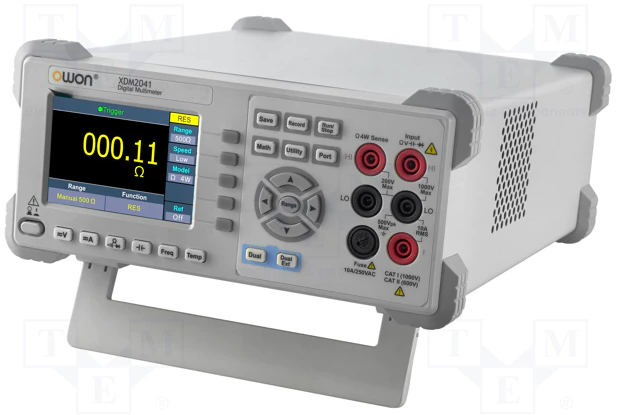
\includegraphics[width=0.4\linewidth, height=0.3\textwidth]{figs/dmm.png}
    \caption{Ejemplo de DMM. Fuente: \cite{DMM}}
    \label{fig:DMM-malo}.
\end{figure}

Debido precisamente a la complejidad ya mencionada, este tipo de mediciones se realizará sobre el cable de alimentación, y no sobre componentes directos, debido a que en este último escenario se requiere desensamblar los componentes, conocer los valores de resistencias, capacitores, etcétera, además de necesitar más instrumental para poder realizar mediciones, como un osciloscopio. 

Los autores de \cite{soton393728} y \cite{soton418538} realizaron un análisis intensivo sobre un \ac{SBC} ODROID-XU3, de la marca Hardkernel, con arquitectura \ac{ARM} Cortex-A53, obteniendo valores de capacitancia y factor de actividad de los componentes de dicha plataforma. Los datos obtenidos de estos artículos se han utilizado como base para el modelo de energía propuesto en este \ac{TFM}, debido al desconocimiento de estos valores en el modelo de pruebas escogido, y a que ambos modelos de pruebas son considerablemente parecidos entre sí, ambos \ac{SBC}s basados en núcleos \ac{ARM} modernos.


\subsection{Análisis vía simulaciones del \textit{hardware}}
\label{sec:Gem5-qemu-estado-arte}
Se entiende por simulación \textit{hardware} a aquellas simulaciones que permiten realizar una réplica relativamente fiable de un sistema a nivel de componentes; esto es, realizar una evaluación de una réplica del sistema a nivel funcional y de arquitectura. De esta forma, es posible el realizar estimaciones de tiempo de forma más precisa que utilizando medidas de tiempo dadas por el sistema operativo, como el contador de tiempo UNIX. En este nuevo esccenario, es posible no solo simulaciones funcionales de programas para observar su rendimiento, sino que además es posible obtener un gran número de métricas procedentes de más bajo nivel que aquellas que pueden ser obtenidas por medio del sistema operativo o de \textit{frameworks} integrados dentro del \textit{kernel}, los cuales son capaces de obtener ciertos eventos, pero están limitados a aquellos que sean interpretables gracias a las capacidades del propio procesador y/o de su arquitectura, como los eventos \textit{hardware} visibles para el sistema operativo: por ello el campo de las simulaciones es especialmente interesante para poder modelar energéticamente una plataforma, especialmente si no se tiene una referencia previa del coste energético de la plataforma. En este contexto, realizar pruebas mediante simulaciones puede ser de gran ayuda, y se emplearán en el desarrollo de este \ac{TFM}. La idea de las simulaciones \textit{hardware} no es precisamente nueva: desde el inicio, las empresas más punteras en el sector de los semiconductores tenían sus propios simuladores privados para probar y validar sus arquitecturas previo lanzamiento al público, permitiendo pulir la tecnología y su fiabilidad en la vida real. 

\subsubsection{qEMU}
\label{subs:qemu}
El primero de los simuladores de código abierto utilizados a gran escala fue qEMU, aunque más bien fue un \textit{software} de \ac{VM}. Esto es relevante, porque determina que al crear un sistema con arquitectura \ac{RISC}, en realidad lo que sucedía era que se creaba una plataforma, completamente abstracta al usuario, comparable a un entorno \textit{chroot} que emula un sistema nuevo, cuando no era así. Aún así, era posible sacar ciertas métricas, (ciclos, inestrucciones ejecutadas, etcétera) que la competencia no era capaz en su tiempo, pero con un sobrecoste considerable por parte de la propia infraestructura de virtualización. Dentro de este \ac{TFM} se ha considerado su uso debido a la simplicidad para obtener métricas relevantes de energía.

Con el paso del tiempo, han surgido un gran número de opciones \textit{open-source} más enfocadas a la simulación de parte de los componentes \textit{hardware} de una plataforma, como el dspliegue de trabajos en procesador (\textit{GEMS}) \cite{PHILLIPS1979225}, o para comprobaciones de la entrada/salida y la memoria principal (\textit{M5}) \cite{10.1109/MM.2006.82}. Precisamente estos dos proyectos, en el año 2011, se fusionaron, dando lugar al simulador Gem5. Este simulador pretende realizar una plataforma personalizada desde cero, sobre la cual el usuario puede agregar y modificar cada componente de forma individual, permitiendo simular con mayor precisión una plataforma real. 

\subsubsection{Comparativa}

Dentro de este trabajo, serán Gem5 y qEMU las opciones tenidas en cuenta. Finalmente, se presenta un análisis detallado de estos dos simuladores, enfocándose en sus fortalezas y debilidades, en la tabla ~\ref{tab:fortalezas_debilidades}.

\begin{table}[H]
    \footnotesize
    \centering
        \begin{tabular}{|c|c|c|}
        \hline
        \rowcolor[HTML]{9B9B9B} 
        \textbf{SIMULADOR} & \textbf{FORTALEZAS} & \textbf{DEBILIDADES} \\ \hline
        \cellcolor[HTML]{EFEFEF} & \begin{tabular}[c]{@{}c@{}}Flexibilidad para simular \\ arquitecturas y sistemas\end{tabular} & Complejidad de uso \\ \cline{2-3} 
        \cellcolor[HTML]{EFEFEF} & \begin{tabular}[c]{@{}c@{}}Modelado detallado de \\ arquitecturas hardware\end{tabular} & \begin{tabular}[c]{@{}c@{}}Rendimiento lento \\ en simulaciones detalladas\end{tabular} \\ \cline{2-3} 
        \cellcolor[HTML]{EFEFEF} & \begin{tabular}[c]{@{}c@{}}Gran escalabilidad hasta \\ sistemas multinúcleo\end{tabular} & \begin{tabular}[c]{@{}c@{}}ARM oculta información necesaria\\ para modelar con precisión\end{tabular} \\ \cline{2-3} 
        \cellcolor[HTML]{EFEFEF} & \begin{tabular}[c]{@{}c@{}}Facilidad para añadir \\ funcionalidades y modelos\end{tabular} & Curva de aprendizaje considerable \\ \cline{2-3} 
        \multirow{-5}{*}{\cellcolor[HTML]{EFEFEF}\textbf{Gem5}} & \begin{tabular}[c]{@{}c@{}}Comunidad activa y \\ actualizaciones periódicas\end{tabular} & Mala integración con IDEs \\ \hline
        \cellcolor[HTML]{EFEFEF} & \begin{tabular}[c]{@{}c@{}}Simulaciones muy rápidas \\ en cualquier situación\end{tabular} & \begin{tabular}[c]{@{}c@{}}Poca flexibilidad \\ y extensibilidad\end{tabular} \\ \cline{2-3} 
        \cellcolor[HTML]{EFEFEF} & \begin{tabular}[c]{@{}c@{}}Compatibilidad con\\ múltiples arquitecturas\end{tabular} & \begin{tabular}[c]{@{}c@{}}Baja precisión \\ en simulaciones detalladas\end{tabular} \\ \cline{2-3} 
        \cellcolor[HTML]{EFEFEF} & Facilidad de uso & \begin{tabular}[c]{@{}c@{}}Las métricas obtenidas \\ poseen mucho ruido\end{tabular} \\ \cline{2-3} 
        \multirow{-4}{*}{\cellcolor[HTML]{EFEFEF}\textbf{qEMU}} & Buena integración con IDEs & Orientado a la funcionalidad \\ \hline
        \end{tabular}
    \caption{Fortalezas y Debilidades de Gem5 y qEMU}
    \label{tab:fortalezas_debilidades}
\end{table}

\subsubsection{Conceptos fundamentales}
\label{subs:conceptos-simulaciones}
Dentro del área de las simulaciones \textit{hardware}, es necesario comprender una serie de términos relevantes en el contexto de este \ac{TFM}:

\par{El \textbf{procesador}, también conocido por \ac{CPU}, es el componente principal de un sistema de cómputo, cuya función es ejecutar instrucciones y procesar datos, utilizando para ello un conjunto de operaciones aritméticas, lógicas, de control y de entrada/salida. Un procesador está compuesto por múltiples unidades funcionales (como \ac{ALU}, \ac{FPU}, registros, y cachés) que trabajan de manera conjunta para interpretar y ejecutar el código máquina que constituye el \textit{software}. En la actualidad, los procesadores han pasado de ser dispositivos secuenciales a arquitecturas complejas con múltiples núcleos, capaces de procesar instrucciones en paralelo y fuera de orden (\ac{O3}), además del uso de técnicas avanzadas como \textit{pipeline}, \textit{hyperthreading}, predicción de saltos, y unidades vectoriales (\ac{SIMD}), para mejorar la eficiencia y el rendimiento. La gran mayoría de procesadores modernos como el presente en el dispositivo de pruebas en este \ac{TFM}, el \ac{ARM} Cortex-A72, incluyen, al menos en parte, las técnicas mencionadas. Los procesadores pueden ser de múltiples arquitecturas, siendo a día de hoy \ac{CISC} y \ac{RISC} las más importantes, cuya diferencia radica en el conjunto de instrucciones que el procesador utiliza para ejecutar programas. La diferencia principal es que los primeros poseen un \ac{ISA} amplio y variado de instrucciones, pudiendo realizar operaciones complejas en una sola instrucción, mientras que los segundos se basan en un \ac{ISA} más simple y reducido, de forma que cada instrucción realiza una operación básica y sencilla, simplificando el diseño del procesador. En el contexto de este trabajo, solamente la arquitectura \ac{RISC} es de relevancia, siendo la utilizada en los procesadores \ac{ARM}.}

\par{La \textbf{memoria caché} es un tipo de memoria pequeña y alojada \textit{dentro} del procesador. Este factor hace que sea muy apta para almacenar las últimas instrucciones y datos utilizados por el procesador y que por tanto, debido al principio de proximidad, puedan con alta probabilidad requerirse por el programa. Debido a su reducido tamaño, la memoria caché almacena las partes más relevantes del mismo conforme avanza la ejecución del programa en el tiempo, lo que obliga al borrado de elementos antiguos para poder almacenar otros nuevos. Para no ralentizar la ejecución, la memoria caché posee diversas técnicas de reemplazo de elementos, como por ejemplo, una política Random, donde se reemplaza \textit{aleatoriamente} un elemento para dar paso a uno nuevo, o \ac{LRU}, donde es el elemento más antiguo en accederse el que se reemplazará por uno nuevo.}

\par{Las \textbf{unidades de cálculo} son componentes esenciales de un procesador que se encargan de realizar operaciones matemáticas y lógicas. Las unidades de cálculo tenidas en consideración en este \ac{TFM} han sido las unidades de cálculo de entero y las unidades de punto flotante. Estas dos unidades son cruciales para el funcionamiento de un procesador moderno, incluyéndose los procesadores \ac{ARM} empleados en este trabajo. Las características principales de ambas son:

\begin{itemize}
      \item \textbf{\ac{ALU}}: encargada de realizar operaciones aritméticas (suma, resta, multiplicación, división) y de operandos lógicos de tipo \emph{AND}, \emph{OR}, \emph{XOR} o \emph{NOT}. Esta unidad es fundamental para diversas tareas informáticas, como la gestión de memoria, la aritmética de direcciones, el control de flujo de programas y la manipulación de datos básicos.
    
      \item \textbf{\ac{FPU}}: encargada de realizar operaciones aritméticas (suma, resta, multiplicación, división) en números de punto flotante, para aquelos números reales con parte entera y parte decimal, como suma, resta, multiplicación, división y operaciones más complejas como raíz cuadrada, logaritmo y funciones trigonométricas. A diferencia de las \ac{ALU}, que trabajan con enteros y operaciones lógicas, las \ac{FPU} manejan números con precisión variable. Esta característica es clave para cálculos científicos o gráficos por computador, entre otros.
\end{itemize}
}

\subsubsection{Métricas importantes}
\label{metricasGem5PAPI}
Debido a las diferencias de \ac{PAPI} y Gem5, las métricas más relevantes y a tener en cuenta tendrán nomenclaturas distintas, siendo para \ac{PAPI} los nombres que poseen los propios eventos de \textit{hardware} recogidos en la documentación oficial \cite{referencia-a72}, mientras que para Gem5 serán los aportados por el generador de estadísticas integrado en el propio \textit{software}. La tabla~\ref{tab:eventosDescPapiGem5} presenta una tabla de las métricas en \ac{PAPI} y su equivalente en el simulador Gem5~\ref{tab:eventosDescPapiGem5}.

\begin{table}[H]
\footnotesize
\centering
\begin{tabular}{|cccc|}
\hline
\rowcolor[HTML]{C0C0C0} 
\multicolumn{4}{|c|}{\cellcolor[HTML]{C0C0C0}\textbf{EQUIVALENCIA MÉTRICAS IMPORTANTES Gem5 Y PAPI}}                                                                                                                                                                \\ \hline
\rowcolor[HTML]{EFEFEF} 
\multicolumn{1}{|c|}{\cellcolor[HTML]{C0C0C0}\textbf{COMP.}}     & \multicolumn{1}{c|}{\cellcolor[HTML]{EFEFEF}\textbf{DESCRIPCIÓN}} & \multicolumn{1}{c|}{\cellcolor[HTML]{EFEFEF}\textbf{Gem5}}                    & \textbf{PAPI}                           \\ \hline
\multicolumn{1}{|c|}{\cellcolor[HTML]{EFEFEF}}                        & \multicolumn{1}{c|}{Número de ciclos}                             & \multicolumn{1}{c|}{system.cpu\_cluster..numCycles}                           & CPU\_CYCLES                             \\ \cline{2-4} 
\multicolumn{1}{|c|}{\cellcolor[HTML]{EFEFEF}}                        & \multicolumn{1}{c|}{Instrucciones entero}                         & \multicolumn{1}{c|}{{[}...{]}.committedInstType::IntAlu}                      & INST\_SPEC\_EXEC\_INT                   \\ \cline{2-4} 
\multicolumn{1}{|c|}{\cellcolor[HTML]{EFEFEF}}                        & \multicolumn{1}{c|}{Instrucciones mult.}                          & \multicolumn{1}{c|}{{[}...{]}.committedInstType::IntMult}                     &                                         \\ \cline{2-3}
\multicolumn{1}{|c|}{\cellcolor[HTML]{EFEFEF}}                        & \multicolumn{1}{c|}{Instrucciones división}                       & \multicolumn{1}{c|}{{[}...{]}.committedInstType::IntDiv}                      & \multirow{-2}{*}{INST\_SPEC\_EXEC\_VFP} \\ \cline{2-4} 
\multicolumn{1}{|c|}{\multirow{-5}{*}{\cellcolor[HTML]{EFEFEF}CPU}}   & \multicolumn{1}{c|}{Instrucciones totales}                        & \multicolumn{1}{c|}{{[}...{]}.executeStats0.numInsts}                         & INST\_SPEC\_EXEC                        \\ \hline
\multicolumn{1}{|c|}{\cellcolor[HTML]{EFEFEF}}                        & \multicolumn{1}{c|}{}                                             & \multicolumn{1}{c|}{}                                                         & L1D\_CACHE\_ACCESS                      \\ \cline{4-4} 
\multicolumn{1}{|c|}{\cellcolor[HTML]{EFEFEF}}                        & \multicolumn{1}{c|}{\multirow{-2}{*}{Accesos a caché L1}}         & \multicolumn{1}{c|}{\multirow{-2}{*}{{[}...{]}dcache.overallAccesses::total}} & L1I\_CACHE\_ACCESSES                    \\ \cline{2-4} 
\multicolumn{1}{|c|}{\cellcolor[HTML]{EFEFEF}}                        & \multicolumn{1}{c|}{Fallos escritura L1D}                      & \multicolumn{1}{c|}{{[}...{]}.dcache.WriteReq.misses::total}                  & L1D\_CACHE\_REFILL                      \\ \cline{2-4} 
\multicolumn{1}{|c|}{\multirow{-4}{*}{\cellcolor[HTML]{EFEFEF}CACHÉ}} & \multicolumn{1}{c|}{Accesos a caché L2}                           & \multicolumn{1}{c|}{{[}...{]}.l2.overallAccesses::total}                      & L2D\_CACHE\_ACCESS                      \\ \hline
\end{tabular}
\caption{Descripción de las métricas más importantes y equivalencia en Gem5 y PAPI}
\label{tab:eventosDescPapiGem5}
\end{table}

\section{Benchmark}
\label{sec:benchmark}
Se entiende por \textit{benchmark} a un proceso riguroso de obtención de datos concretos relativos a una plataforma. Este tipo de programas se emplean tras el diseño y modelado de una plataforma \textit{hardware}, con el objetivo de poder dar una evaluación relativa a su desempeño real, pasando (o no) las pruebas pertinentes. En el contexto de este trabajo, se emplearán \textit{benchmarks} de \emph{carácter sintético} (explicados en \label{sec:tipos-benchmark}) con el objetivo de enfocar el esfuerzo en componentes concretos de la plataforma en cuestión. Un \textit{benchmark} ~\cite{benchmarking-concepto} debe ser:

\begin{itemize}
  \item Repetible: es crucial garantizar que las pruebas de referencia se ejecuten de manera consistente y reproducible para obtener resultados confiables.
  \item Comparable: los resultados del benchmarking deben ser comparables con otros sistemas o aplicaciones utilizando metodologías y métricas consistentes.
  \item Validable: Los resultados del benchmarking deben validarse para garantizar que reflejan el rendimiento real del sistema o aplicación en condiciones de uso normal.
\end{itemize}

En la actualidad, existen un gran número de técnicas para comparar el rendimiento de un sistema informático desde sus diferentes puntos de vista. Entre las opciones más utilizadas se encuentran:

\begin{itemize}
  \item Benchmarks de rendimiento: Evalúa la velocidad y la capacidad de respuesta de un sistema o aplicación al realizar tareas específicas.
  \item Benchmarks de consumo de energía: Mide el consumo de energía de un sistema o dispositivo bajo diferentes cargas de trabajo.
  \item Benchmarks de escalabilidad: Analiza cómo el rendimiento de un sistema se ve afectado al aumentar la carga o el número de usuarios.
  \item Benchmarks de comparación: Compara el rendimiento de un sistema o aplicación con el de otros productos o soluciones competitivas.
\end{itemize}

Existen numerosas herramientas de benchmarking disponibles para realizar pruebas y análisis de rendimiento. 
En el contexto de este trabajo se ha optado por el uso de herramientas gratuitas en su totalidad, lo que ha impedido el empleo de gran cantidad de \textit{benchmarks} conocidos, como la suite de programas \ac{SPEC} versión 2006 y \ac{SPEC} versión 2017 \cite{spec2006} \cite{spec2017}, ya que se requiere de una licencia para poder utilizarlos. En su lugar, se han realizado los \textit{benchmarks} utilizando programas desarrollados en el lenguaje de programación C, los cuales cada uno se centra en un aspecto concreto del sistema. El sitio de obtención del código fuente de estos programas ha sido Netlib ~\cite{netlib-library}

A la hora de seleccionar un \textit{benchmark}, existen numerosas opciones a elegir, dependiendo de los componentes que se quieran valorar. En el contexto de este \ac{TFM}, será unicamente el componente procesador el que será evaluado. Las razones de esta decisión son variadas, siendo la principal de todas ellas la gran dificultad que supondría representar en un simulador \textit{hardware} una aplicación real, por ejemplo, sobre la detección de objetos con OpenCV mediante el uso de una red neuronal. Esto obligaría a compilar librerías externas de C como OpenCV y TensorFlow para una plataforma, que si bien se asemeja a una real, no es completamente igual, y podría carecer de ciertos componentes, y configuraciones necesarias para que la aplicación se ejecutara correctamente. 

Finalmente, dentro del contexto de este \ac{TFM}, los \textit{benchmarks} que se han tenido en cuenta son:

\begin{enumerate}
  \item \textbf{Dhrystone}: Dhrystone es un \textit{benchmark} de referencia que mide el rendimiento de entero de un sistema, ejecutando operaciones matemáticas simples y estructuras de control de flujo. En Dhrystone, las cargas de trabajo se miden en instrucciones Dhrystone, instrucciones de código máquina sintéticas diseñadas para representar un conjunto de instrucciones intensivas en ALU comunes en programas científicos.
  
  \item \textbf{Whetstone}: fruto de la evolución de la computación y la adición de unidades de punto flotante a los procesadores, surge el \textit{benchmark} Whetstone, el cual mide el rendimiento de punto flotante, ejecutando cálculos científicos y de ingeniería complejos. Al igual que en Dhrystone, en Whetstone se representan las cargas de trabajo con instrucciones Whetstone, siendo en este caso instrucciones intensivas en FPU comunes en programas científicos.
  
  \item \textbf{Cálculo de números primos, método Miller-Rabin}: el cáculo de números primos pretende medir el rendimiento de la comunicación entre RAM y memorias caché del sistema, además de las unidades \ac{ALU} y \ac{FPU}, esta última en menor medida. Las cargas de trabajo se definen por la cantidad de números sobre los que se deberá comprobar si cada uno es primo o no en cada ejecución del textit{benchmark}.
  
  \item \textbf{Cálculo de decimales del número Pi, método Gauss-Legendre}: el cálculo de decimales del número Pi pretende medir, al igual que en el punto anterior, caché, RAM, y rendimiento de las unidades \ac{ALU} y \ac{FPU}, siendo especialmente ésta última a la que está orientado este \textit{benchmark}. Las cargas de trabajo se definen por el número de decimales de Pi que será necesario averiguar en cada ejecución del textit{benchmark}.
\end{enumerate}